\section{Results}

This section provides an overview of the results from my method. 

\subsection{Overall Measures}

% shows the mean fairness and compactness measures for the redistricting plans generated by the two algorithms and the existing congressional districts. 

% For the Edge-Cut Compactness and Fryer-Holden score, the table contains the mean of the respective measures for the 100 plans generate by the algorithms. For the Polsby-Popper score, the table contains the mean of the district-level mean Polsby-Popper score for all 100 plans. The compactness measures were normalized so that values of 1 indicate more compact districts and values of 0 represent the least compact districts. 

% The fairness measures in the table are all the mean of said fairness measure for each redistricting plan generated by each algorithm. "dseats" is the average number of seats that Democrats would have held had the 2018 General Election taken place with said redistricting plan. All other remaining fairness measures have been normalized, where values of 0 indicate fairness and deviation in either direction indicates a partisan imbalance. 

\subsection{Compactness}
\begin{figure}
    \centering
    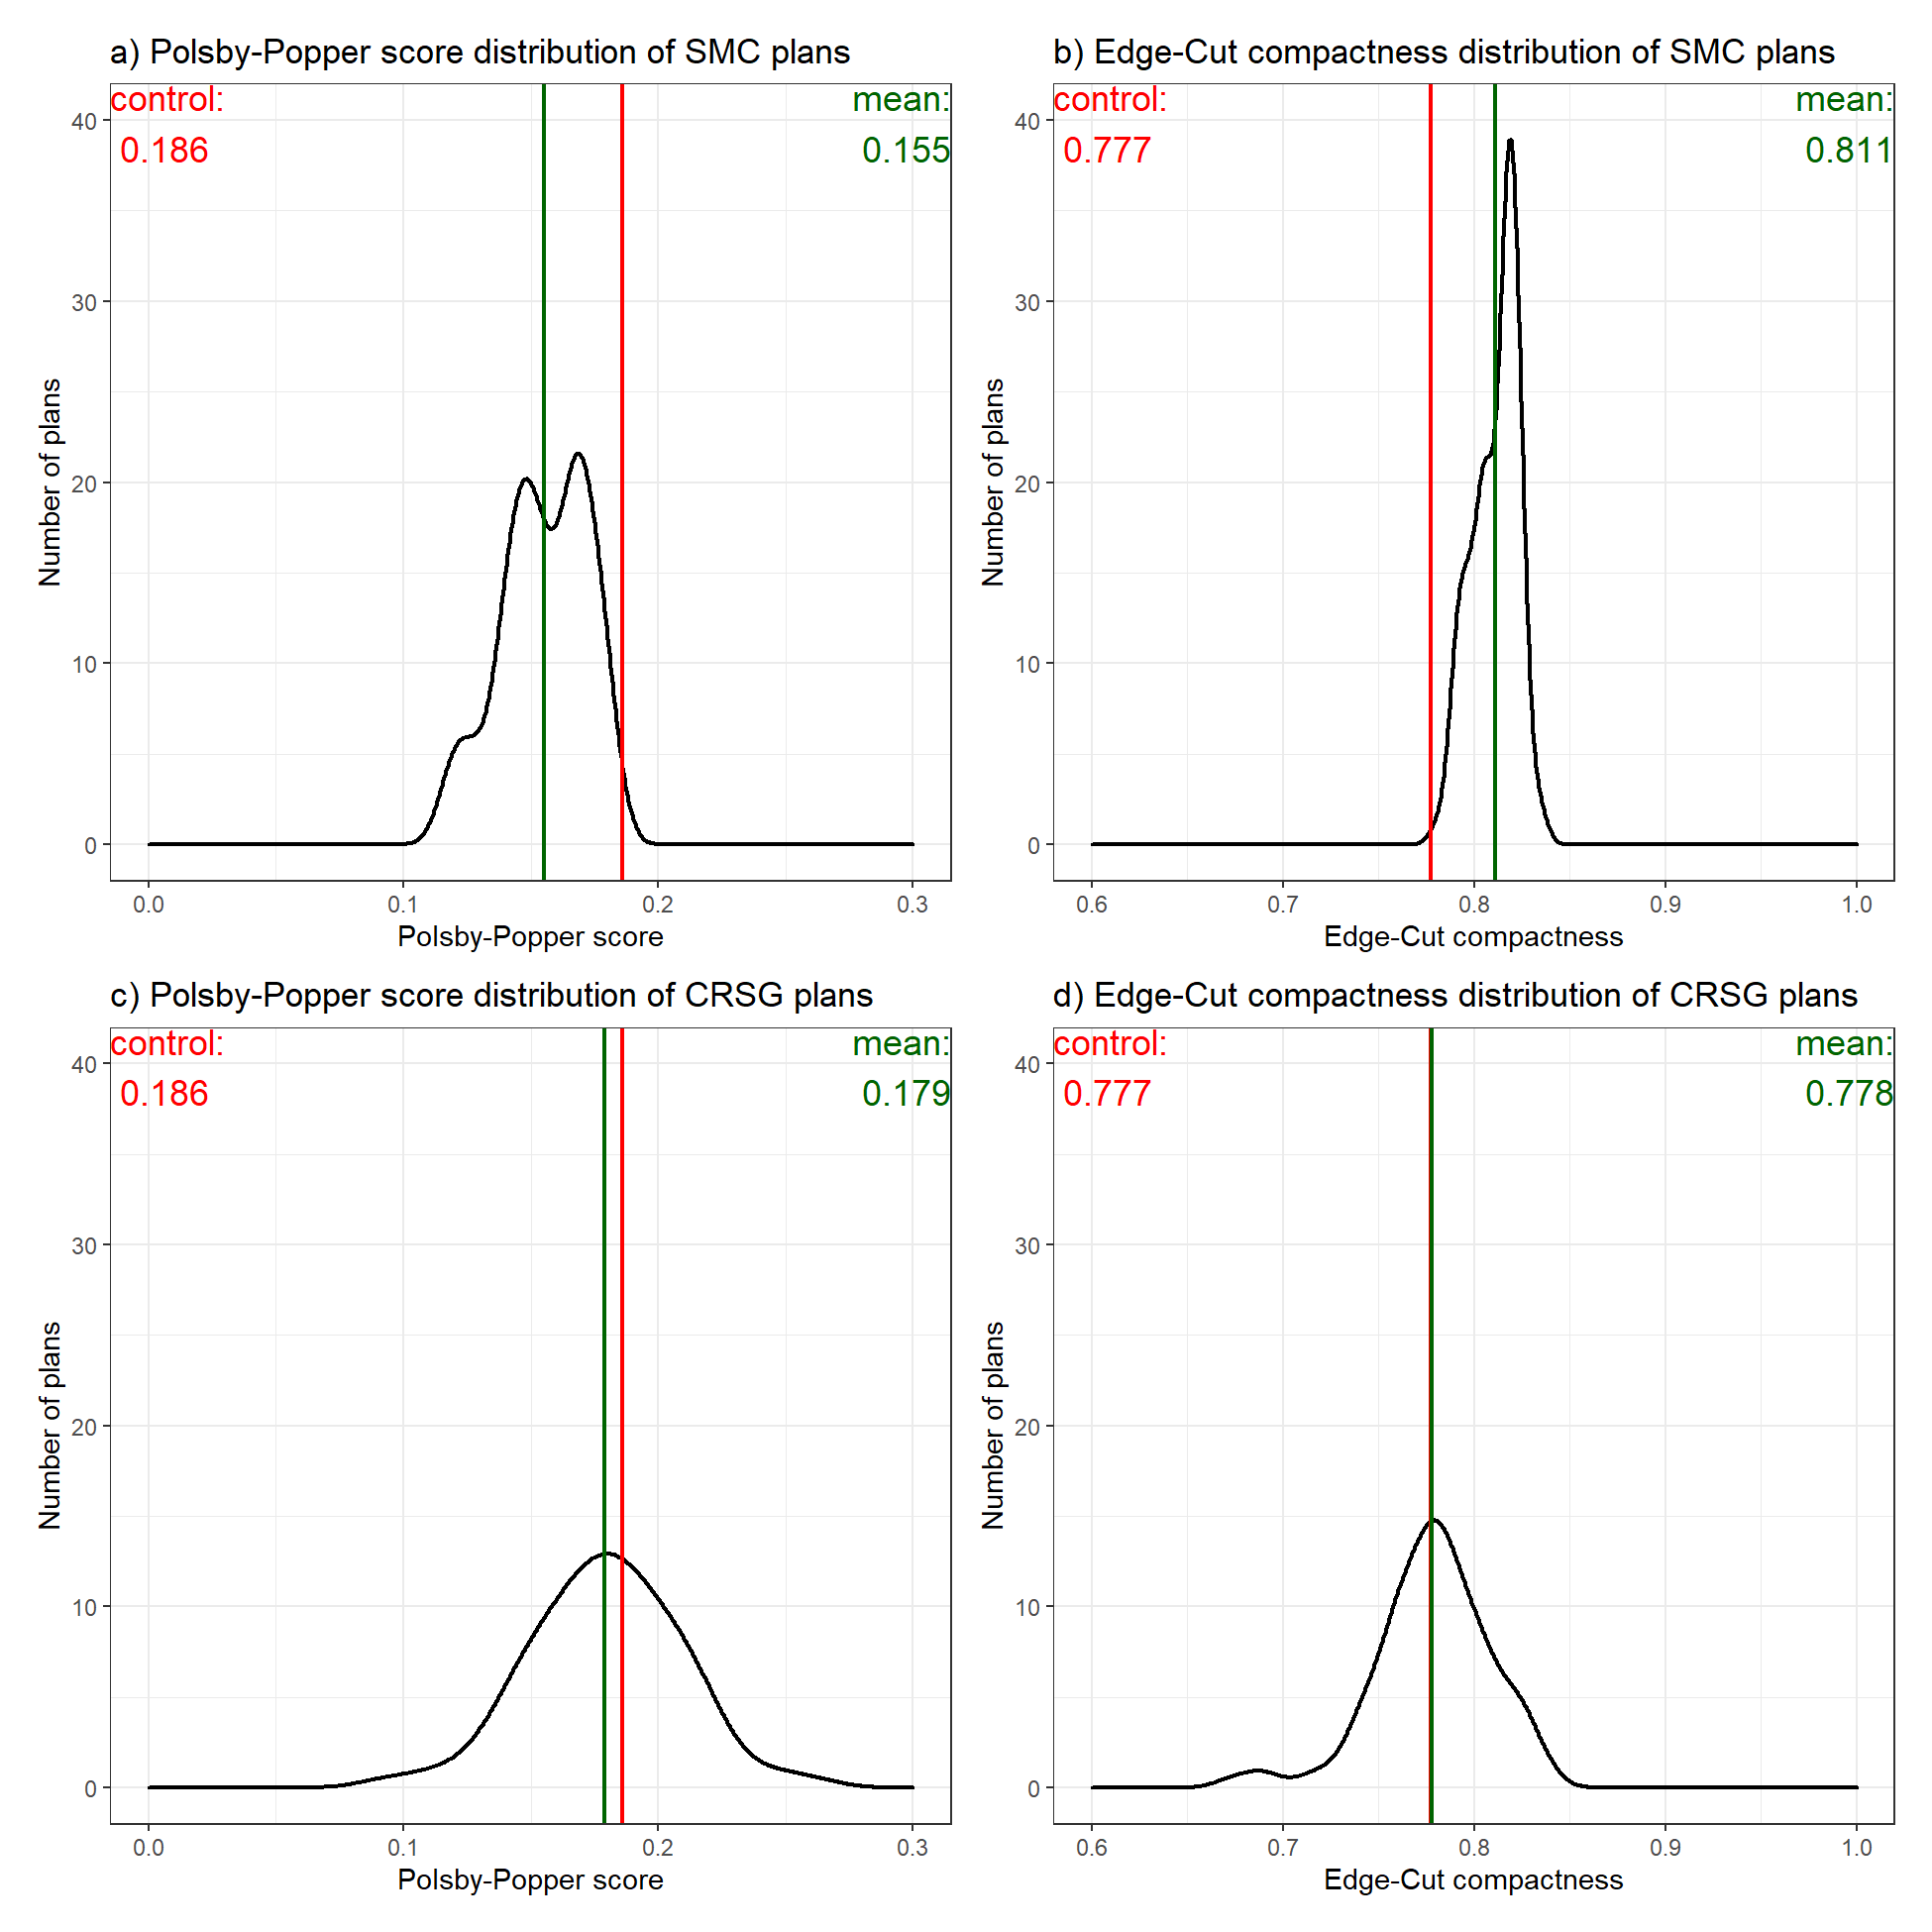
\includegraphics[width=\textwidth]{img/compact.density.png}
    \caption{Distributions of compactness measures.}
    \label{fig:compact.density}
\end{figure}

% REWRITE THIS
% Figure \ref{fig:compact_hist} visualizes districts of varying compactness levels. Subfigure \ref{fig:map.mcmc.pp} illustrates the redistricting plan generated by MCMC with the greatest average Polsby-Popper score. Subfigure \ref{fig:map.mcmc.ec} shows the corresponding plan from MCMC with the greatest Edge-Cut Compactness score. Subfigures \ref{fig:map.smc.pp} and \ref{fig:map.smc.ec} illustrate the corresponding redistricting plans satisfying the same requirements but generated by SMC. The existing district map of Virginia is illustrated by \ref{fig:map.control} for reference. 

\subsection{Partisan Fairness}
\begin{figure}
    \centering
    \begin{subfigure}[b]{0.475\textwidth}
        \centering
        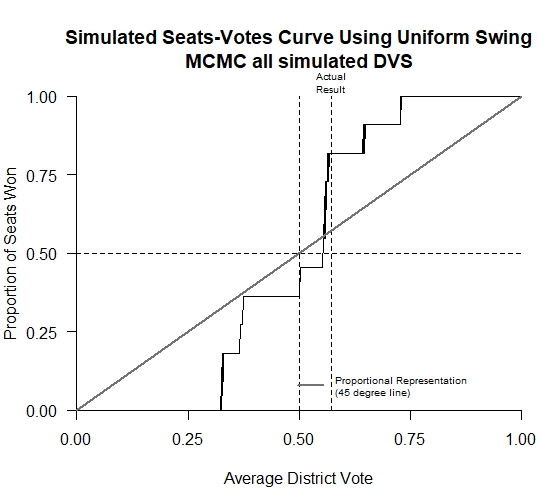
\includegraphics[width=\textwidth]{img/sv.mcmc.png}
        \caption{MCMC Seats-Votes Curve}
        \label{fig:sv.mcmc}
    \end{subfigure}
    \hfill
    \begin{subfigure}[b]{0.475\textwidth}
        \centering
        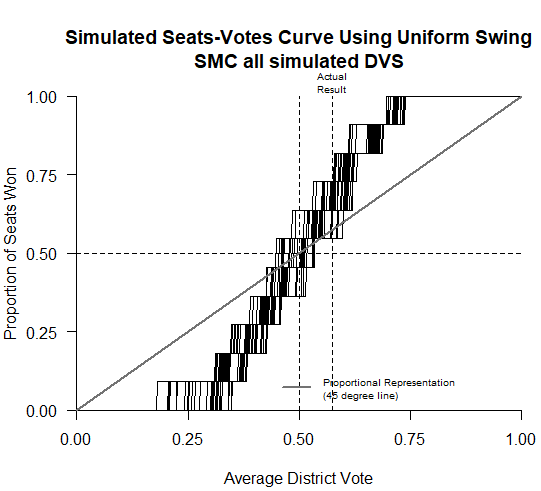
\includegraphics[width=\textwidth]{img/sv.smc.png}
        \caption{SMC Seats-Votes Curve}
        \label{fig:sv.smc}
    \end{subfigure}
    \vskip\baselineskip
    \begin{subfigure}[b]{0.475\textwidth}
        \centering
        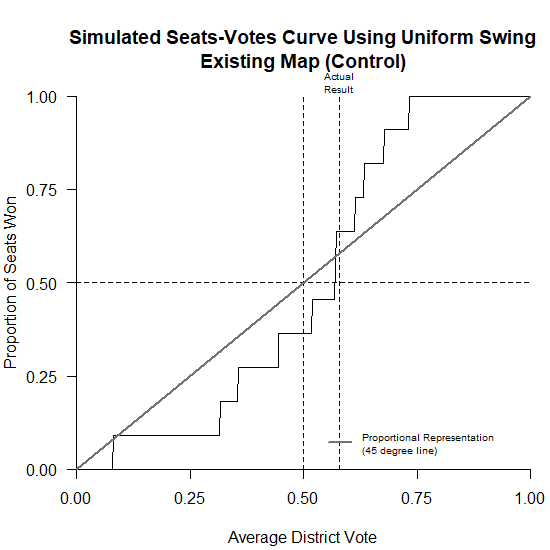
\includegraphics[width=\textwidth]{img/sv.control.png}
        \caption{Real Seats-Votes Curve}
        \label{fig:sv.control}
    \end{subfigure}
       \caption{Seats Votes Curves}
       \label{fig:sv}
\end{figure}

% REWRITE THIS  
% Figure \ref{fig:sv} shows the seats-votes curves \parencite{katz2020} for the 2018 General Election under the redistricting plans generated by both algorithms and the existing map. For each plot, the x-axis plots the average of the proportion of votes won by Democrats in each district. The y-axis plots the proportion of seats won by Democrats in the delegation. Both subfigures \ref{fig:sv.mcmc} and \ref{fig:sv.smc} have once curve for each redistricting plan (each plot has 100 curves). The seats-votes curve for the real 2018 districts is provided for reference in subfigure \ref{fig:sv.control}.

\begin{landscape}
    \begin{figure}
     \centering
     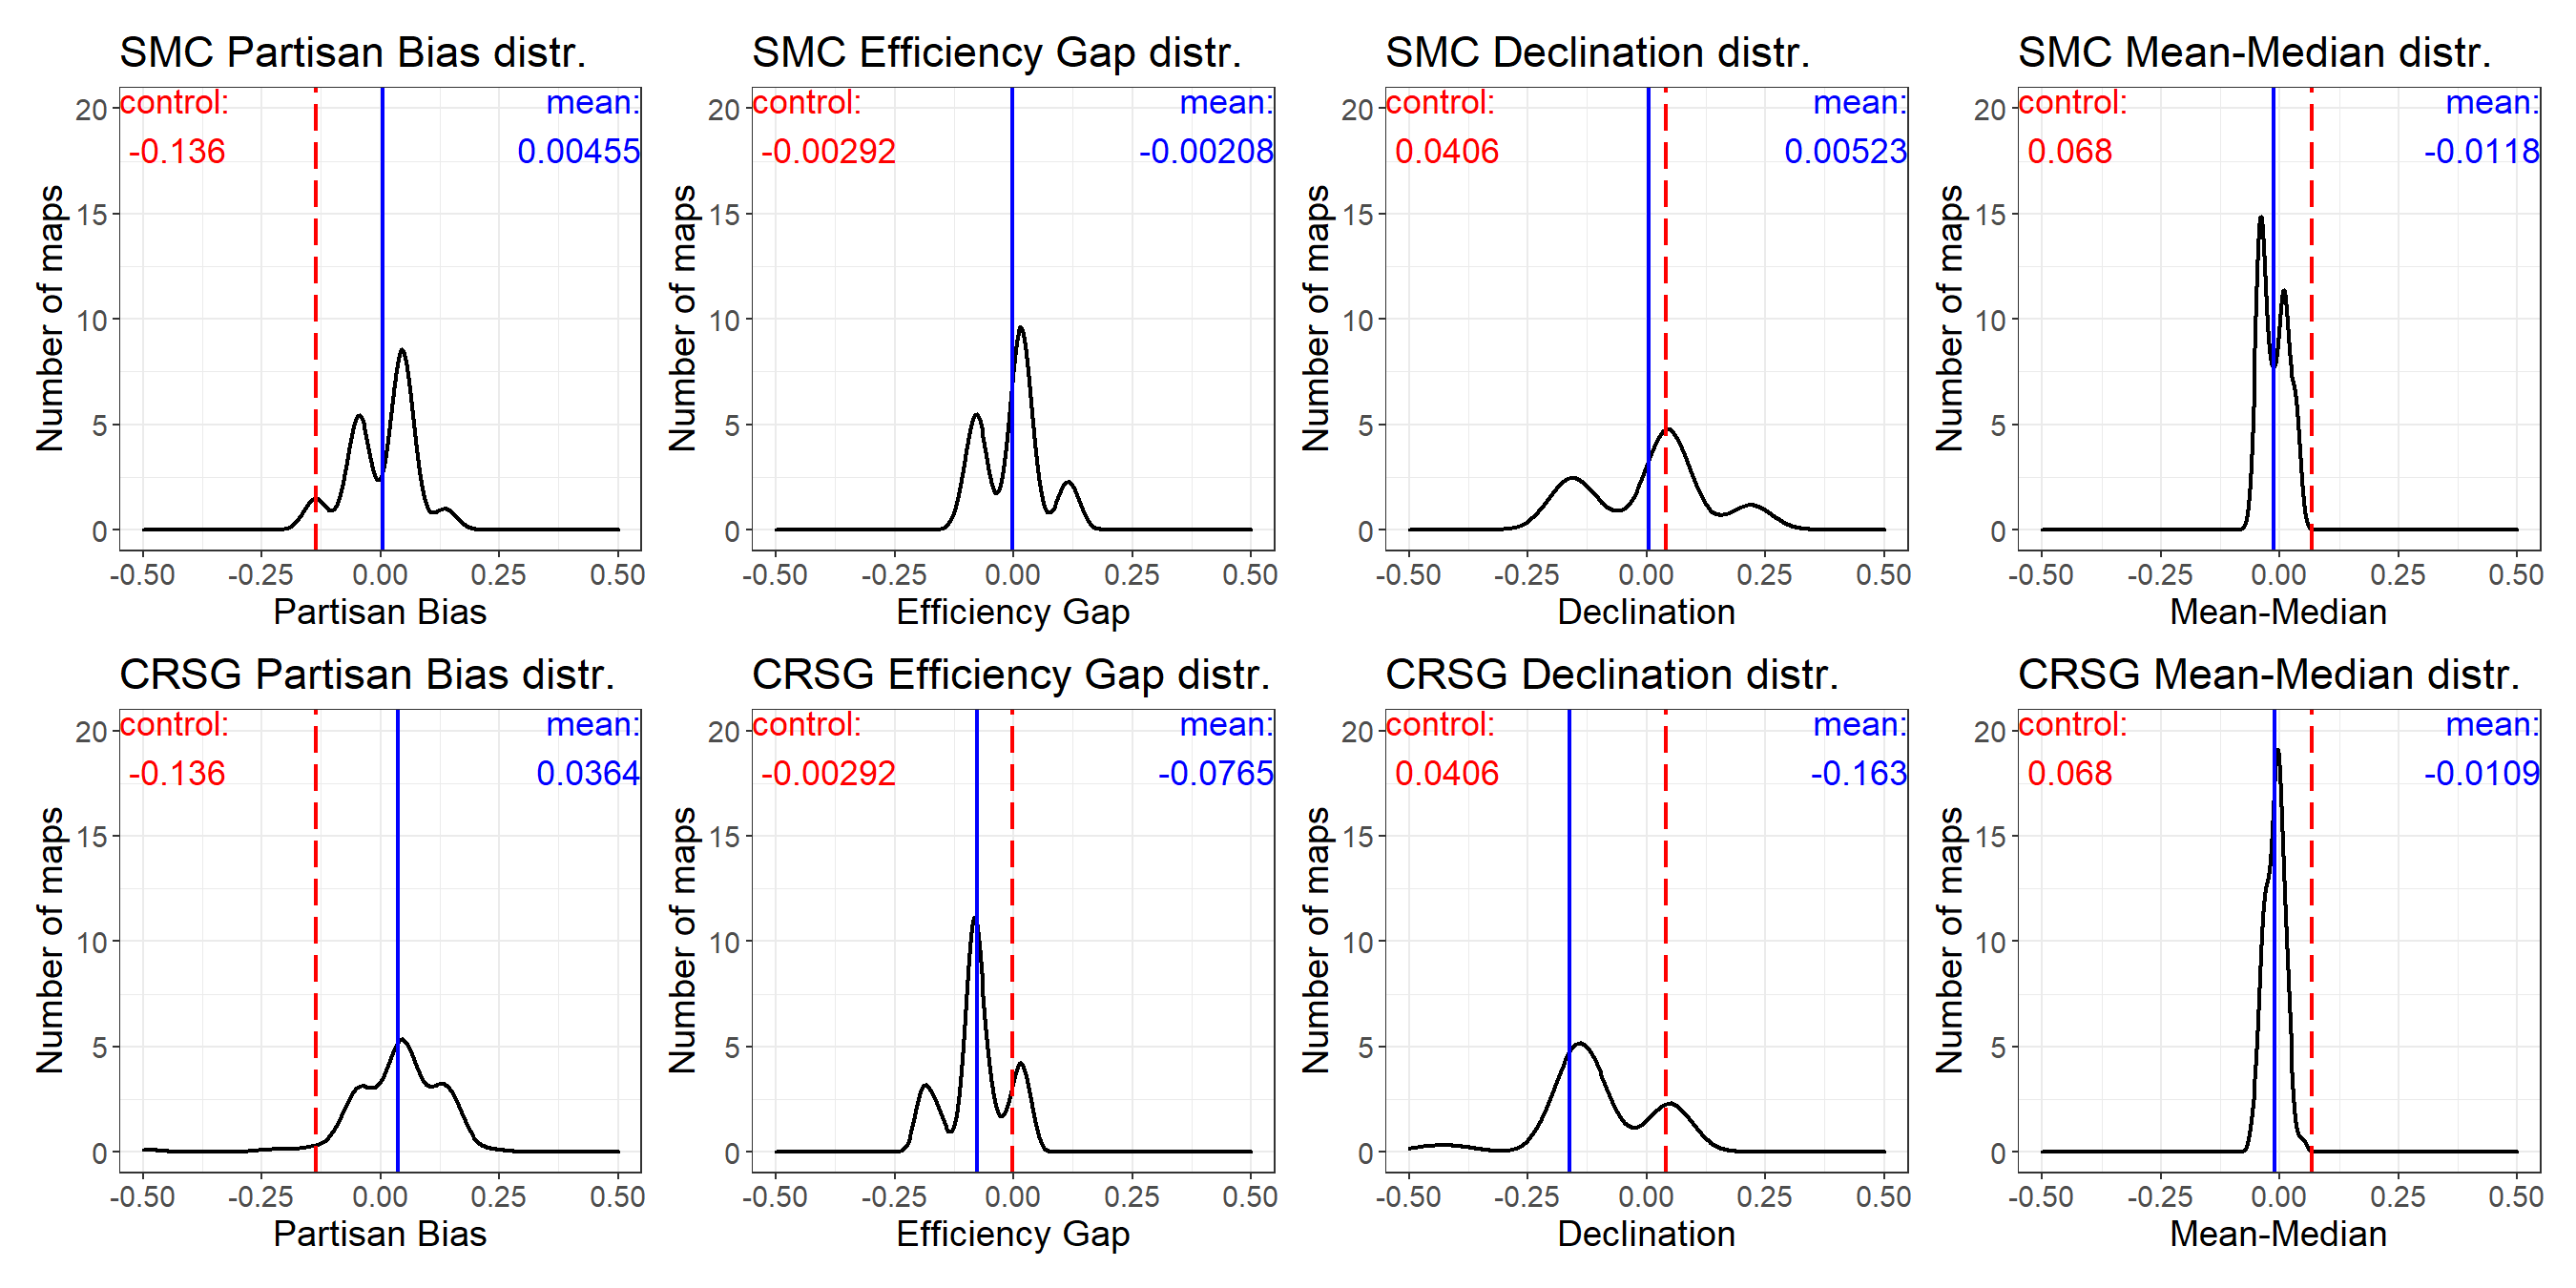
\includegraphics{img/fair.density.png}
     \caption{Distributions of fairness measures}
     \label{fig:fair.density}
    \end{figure}
   \end{landscape}

\subsection{2018 General Election Simulation}
\begin{figure}
    \centering
    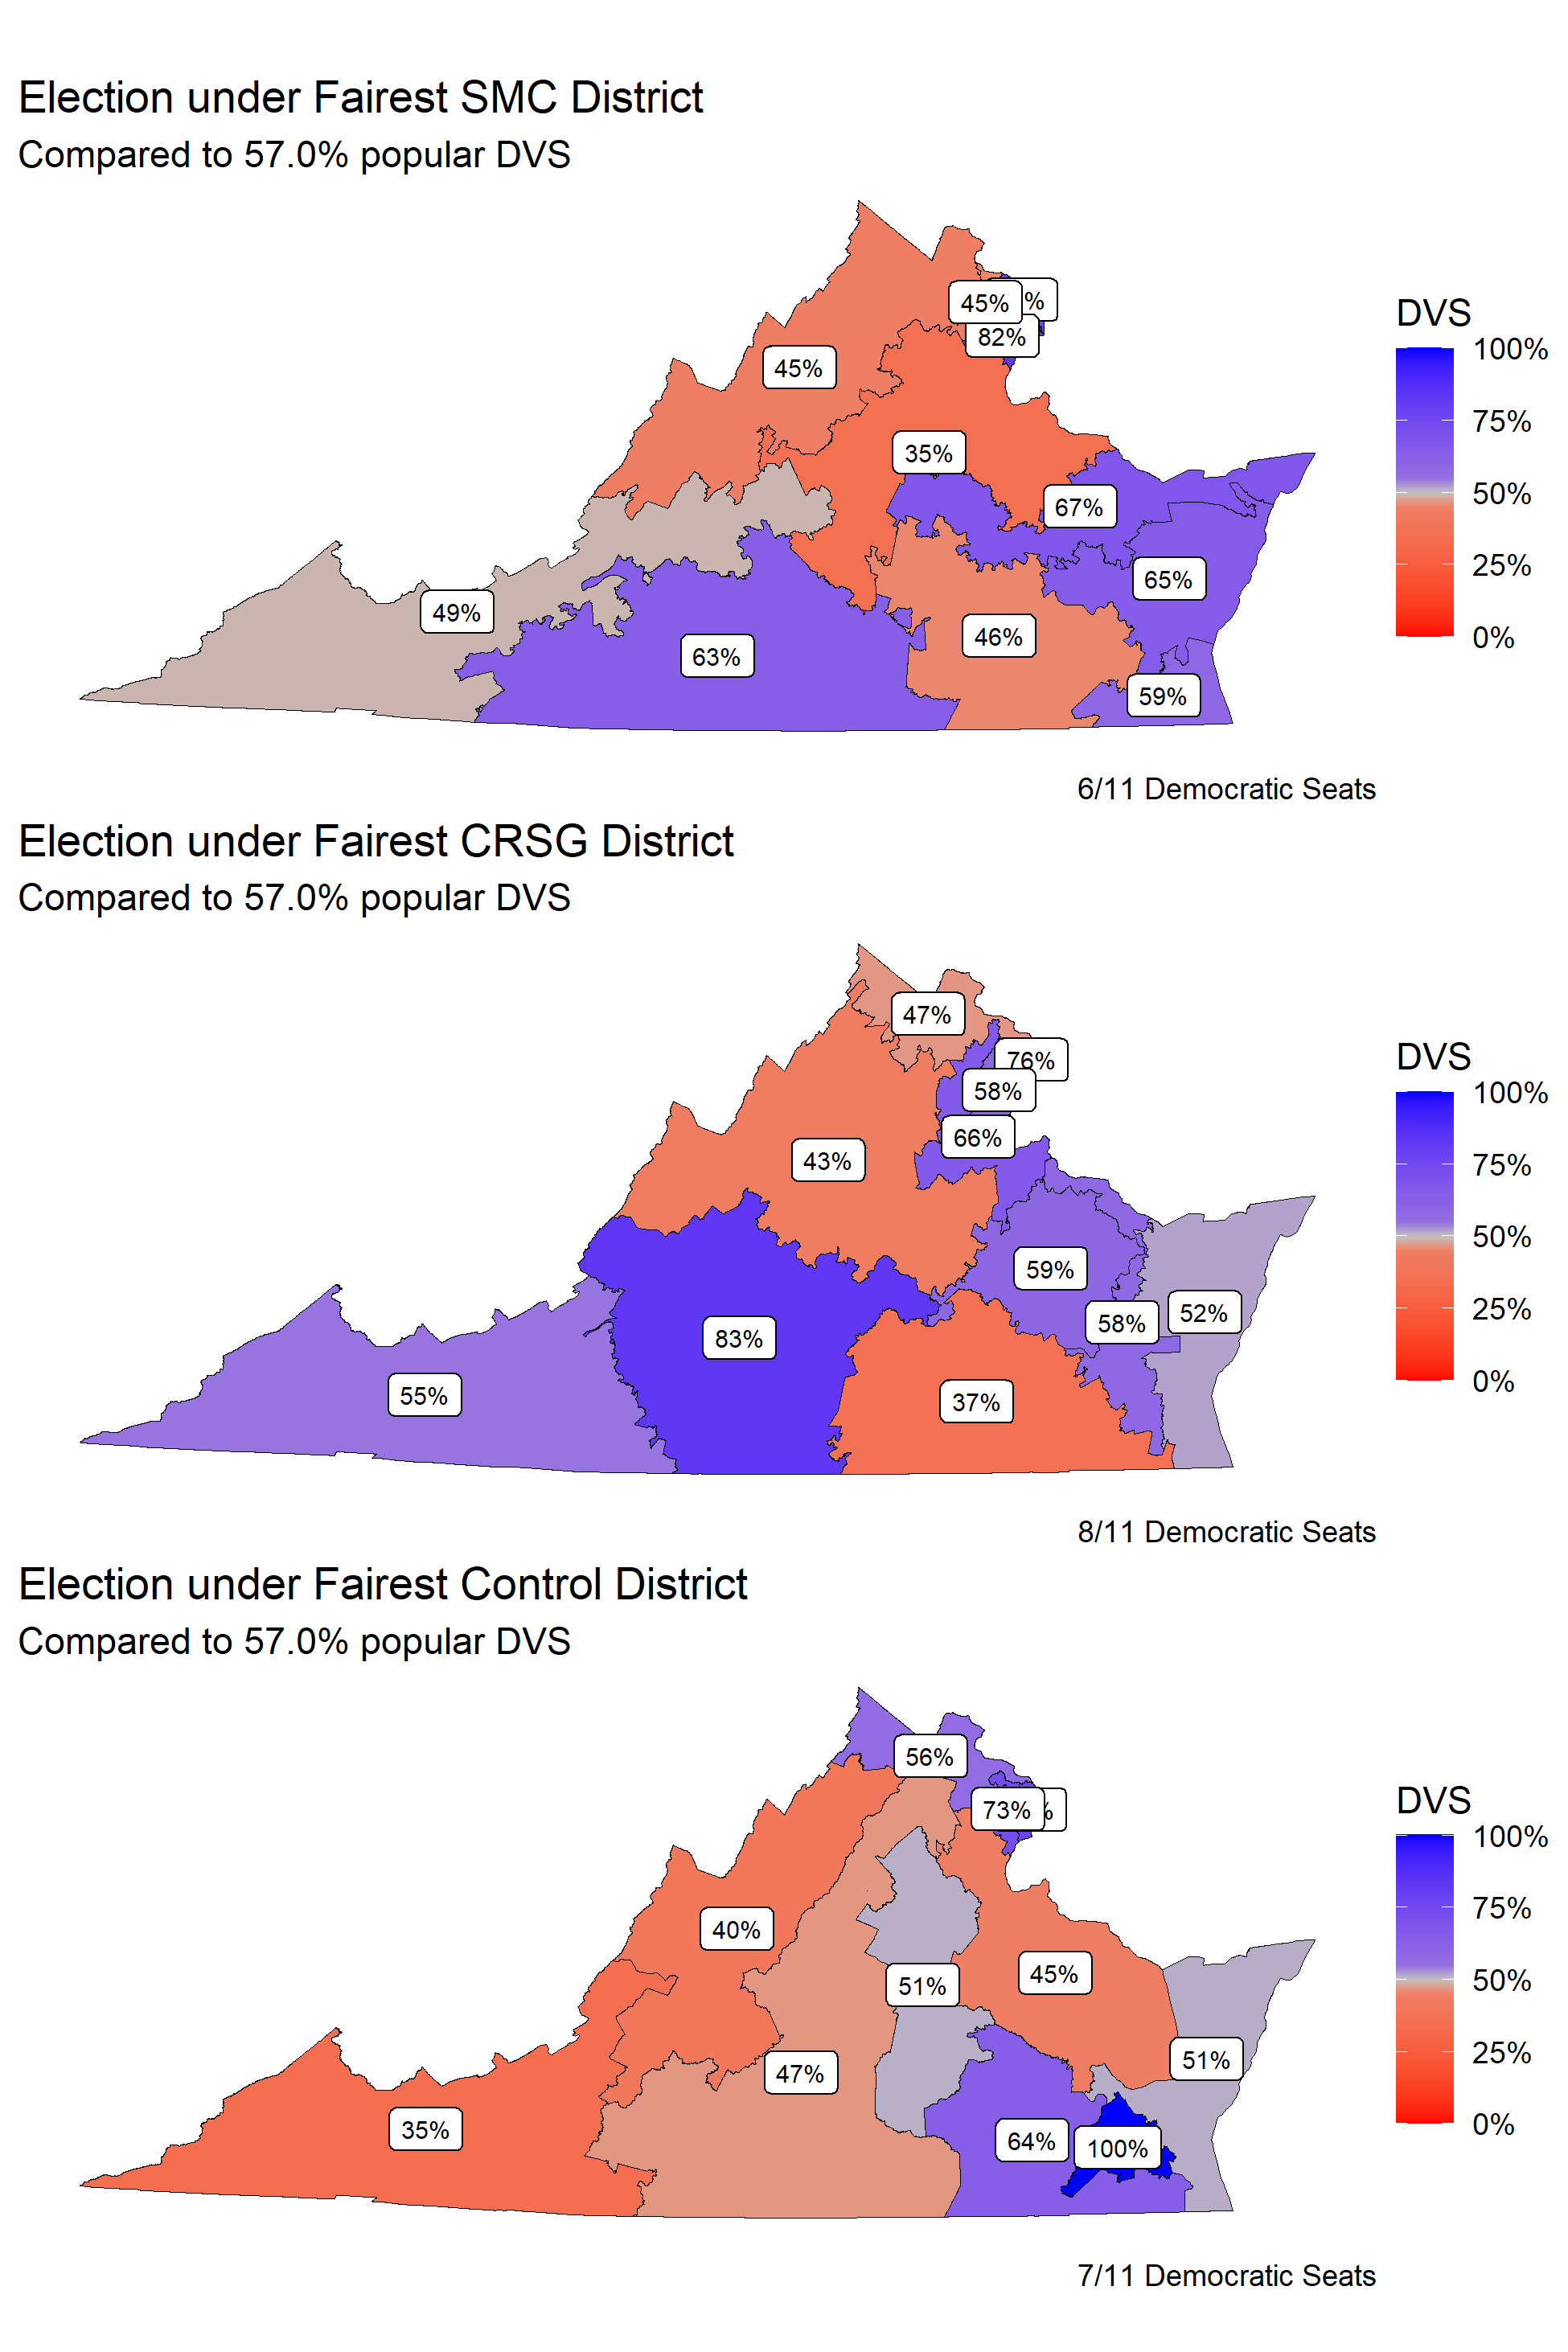
\includegraphics[width=0.8\textwidth]{img/election.map.png}
    \caption{Simulated election results}
    \label{fig:election.map}
\end{figure}

% Figure \ref{fig:elec} visualizes the outcome of a simulated 2018 General Election under various redistricting plans. Subfigure \ref{fig:elec.mcmc} was created by aggregating the precinct-level election results from 2018 to the district level using the redistricting plan generated by MCMC with the least partisan bias. The average precinct-level proportion of votes won by Democrats in the district is displayed as a percentage. Values closer to 1 indicate a higher proportion of Democratic votes and are colored blue. Values closer to 0 indicate a higher proportion of Republican votes and are colored red. Purple districts are most competitive. Subfigure \ref{fig:elec.smc} illustrates this same simulation, only using the corresponding "fairest" redistricting plan generated by SMC. The real results from the 2018 General Election are visualized in subfigure \ref{fig:elec.control} for reference. 